\ChapterImageStar[cap:pmv]{Producto Mínimo Viable}{./images/fondo.png}\label{cap:pmv}
\mbox{}\\
En este capítulo se implementará el sistema propuesto en la infraestructura HTCondor del Grupo \GRID. Además, se enunciarán las características de cada componente del sistema, su contenido, requisitos y guía de instalación, para hacer un entorno repetible y escalable.

Cabe destacar que para este proyecto se usó Git para el control de versiones, GitHub para gestión de repositorios y se usó un enfoque hacia versionamiento semántico o \textit{SemVer}. Por lo que se mostrarán las aplicaciones y se mencionará la última versión funcional de la aplicación con un \textit{tag}.

\section{\textit{Grid App}}
\noindent
Como se mencionó en el capítulo de diseño de la solución, la aplicación \textit{Grid App} constituye la piedra angular del sistema, pues es este \textit{software} el que permite centralizar la funcionalidad de los demás componentes. El objetivo de esta aplicación es exponer una interfaz web en la que el usuario pueda cargar sus trabajos computacionales, dar ciertos parámetros para su ejecución y que luego pueda ver los resultados de sus trabajos.

\subsection{Estructura del proyecto}
\noindent
La figura~\ref{fig:estructura-proyecto-grid-app} detalla la estructura del proyecto; el directorio \textit{scripts} contiene algunos ejecutables de Bash que usa el sistema para enviar los trabajos al Universo \textit{Parallel} y sincronizar las salidas; el directorio \textit{static} contiene algunos archivos de \CSS~y \JS~útiles para darle forma e interacción a la interfaz web; el directorio \textit{submits} está destinado a guardar los archivos de HTCondor, como los \textit{submit files} y los resultados de los trabajos; el repositorio \textit{templates} contiene el código \HTML~que conforma la estructura de las páginas web y por último; los archivos que están en la raíz del proyecto que son \textit{app.py}, que compone el código del servidor de Python y \textit{.gitignore} que le dice a Git que archivos y carpetas debe ignorar y es común a la mayoría de proyectos que usan este \CVS.

\begin{figure}[H]
	\centering
	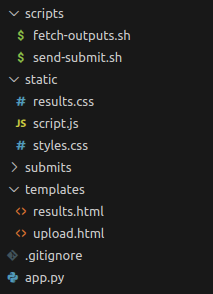
\includegraphics[scale=0.35]{tablas-images/pmv/estructura-proyecto-grid-app.png}
	\caption{Estructura del proyecto \textit{Grid App}}
	\label{fig:estructura-proyecto-grid-app}
\end{figure}

\subsection{Código fuente}
\noindent

El código fuente de la aplicación \textit{Grid App}, está disponible en el repositorio de GitHub \href{https://github.com/JuanEstebanOsma1012/condor\_webui}{\textit{condor\_webui}} en la rama \href{https://github.com/JuanEstebanOsma1012/condor\_webui/tree/main}{\textit{main}} y su versión más actualizada y funcional a la fecha es la \href{https://github.com/JuanEstebanOsma1012/condor\_webui/releases/tag/v3.1.0}{v3.1.0}. De igual forma, en el apéndice XX se muestran los contenidos y la descripción de cada archivo que compone esta aplicación.

\subsection{Componentes de la interfaz web}
\noindent
En esta sección se muestran las interfaces de usuario que sirve la aplicación. Además de la descripción de la utilidad de cada una.

\subsubsection{Upload UI}
\noindent
Es la interfaz de usuario principal de toda la aplicación. Como se muestra en la figura \ref{fig:uiCargasTrabajos} está compuesta por un formulario que permite entregar información sobre el trabajo para su posterior ejecución.

\begin{figure}[H]
	\centering
	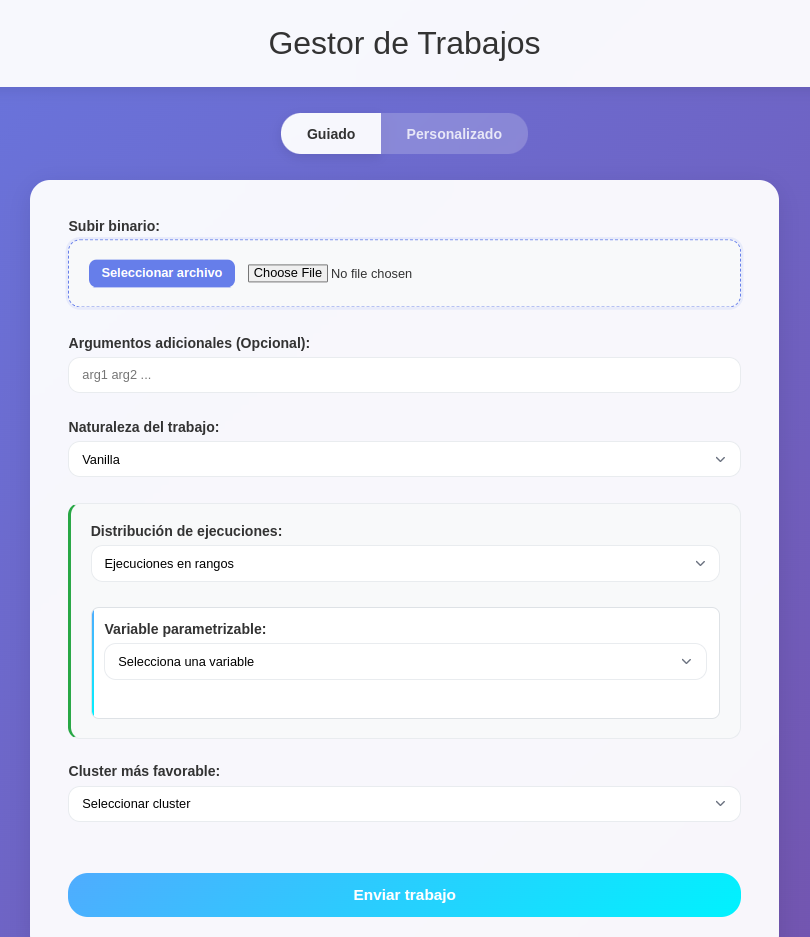
\includegraphics[scale=0.35]{tablas-images/pmv/upload-ui-screenshot.png}
	\caption{Interfaz de carga de trabajos}
	\label{fig:uiCargasTrabajos}
\end{figure}

\subsubsection{Results UI}
En la figura \ref{fig:uiResultadosTrabajos} se muestra la interfaz de los resultados de cada trabajo distribuido. Permite una previsualización del contenido de los resultados de los trabajos y también, permite ampliar la salida completamente. Por último, muestra información general del trabajo como su UUID asignado por el sistema, el nombre del ejecutable y otros datos de interés.

\begin{figure}[H]
	\centering
	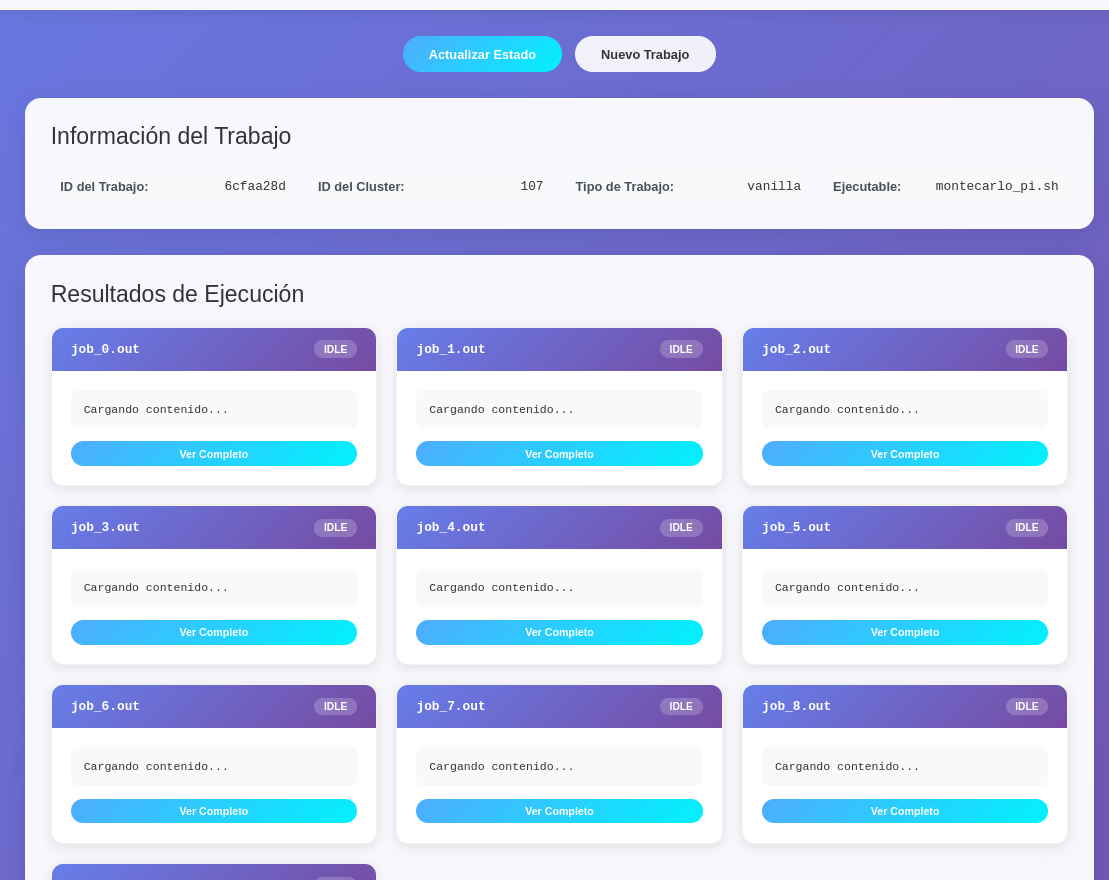
\includegraphics[scale=0.35]{tablas-images/pmv/results-ui-screenshot.png}
	\caption{Interfaz de resultados de trabajos}
	\label{fig:uiResultadosTrabajos}
\end{figure}

\subsection{Componentes Backend (Endpoints)}
\noindent

Los componentes \textit{backend} de \textit{Grid App} están implementados como \textit{endpoints} en Flask y constituyen el núcleo funcional de la aplicación. Estos componentes son responsables de recibir las solicitudes del usuario, procesarlas, interactuar con HTCondor y gestionar el ciclo de vida completo de los trabajos computacionales. A continuación se describe cada uno de los \textit{endpoints} principales del sistema.

\subsubsection{Submit Endpoint}
\noindent

El \textit{Submit Endpoint} es el componente responsable de recibir la información del trabajo computacional a ejecutar y enviarlo al clúster HTCondor correspondiente. Este \textit{endpoint} está expuesto en la ruta \texttt{/submit} y acepta peticiones de tipo POST.

\textbf{Funcionamiento:}

El proceso que ejecuta este componente puede describirse en los siguientes pasos:

\begin{enumerate}
	\item \textbf{Generación del identificador único}: Al recibir una petición, el \textit{endpoint} genera un identificador único (UUID) de 8 caracteres para el trabajo. Este identificador se utiliza para crear un directorio específico dentro de \texttt{/submits/} donde se almacenarán todos los archivos relacionados con el trabajo.
	
	\item \textbf{Procesamiento de archivos}: El componente recibe y procesa tres tipos de archivos opcionales:
	\begin{itemize}
		\item \textit{binary-file}: El archivo ejecutable del trabajo.
		\item \textit{input-file}: Archivo de entrada necesario para la ejecución (principalmente para trabajos paralelos).
		\item \textit{submit-file}: Archivo de configuración personalizado de HTCondor.
	\end{itemize}
	
	\item \textbf{Configuración del trabajo}: El \textit{endpoint} recibe un objeto JSON con la configuración del trabajo que incluye:
	\begin{itemize}
		\item \texttt{jobType}: Tipo de universo (vanilla o parallel).
		\item \texttt{cluster}: Dirección IP y puerto del clúster destino.
		\item \texttt{additionalArgs}: Argumentos adicionales para el ejecutable.
		\item Opciones específicas según el tipo de trabajo.
	\end{itemize}
	
	\item \textbf{Generación del archivo submit}: Si el usuario no proporciona un archivo submit personalizado, el componente genera automáticamente uno basado en la configuración recibida, utilizando la función \texttt{create\_submit\_file()}. Esta función crea archivos submit diferentes según el tipo de universo:
	
	\begin{itemize}
		\item \textbf{Para Universo Grid (Vanilla)}: Genera un archivo submit que especifica el \textit{grid\_resource}, configura la transferencia de archivos y establece los requisitos de arquitectura. Además, maneja dos modos de distribución de trabajos:
		\begin{itemize}
			\item \textit{Modo range}: Genera múltiples trabajos con valores de variables distribuidos en rangos especificados.
			\item \textit{Modo equal}: Genera múltiples trabajos idénticos según el número de repeticiones especificado.
		\end{itemize}
		
		\item \textbf{Para Universo Parallel}: Genera un archivo submit que utiliza el \textit{openmpiscript}, especifica el número de máquinas y núcleos por máquina, configura las variables de entorno para OpenMPI y establece las políticas de transferencia de archivos y apagado.
	\end{itemize}
	
	\item \textbf{Envío al clúster}: Dependiendo del tipo de trabajo, el componente ejecuta diferentes estrategias:
	
	\begin{itemize}
		\item \textbf{Trabajos Vanilla}: Ejecuta directamente el comando \texttt{condor\_submit} sobre el archivo submit generado en el directorio del trabajo.
		
		\item \textbf{Trabajos Parallel}: Invoca el script \texttt{send-submit.sh} que se encarga de transferir los archivos necesarios al clúster remoto mediante SSH y ejecutar \texttt{condor\_submit} en dicho clúster. Adicionalmente, inicia un hilo separado que ejecuta el script \texttt{fetch-outputs.sh} para sincronizar periódicamente los archivos de salida desde el clúster remoto.
	\end{itemize}
	
	\item \textbf{Extracción del cluster ID}: El componente analiza la salida del comando \texttt{condor\_submit} utilizando expresiones regulares para extraer el número de clúster asignado por HTCondor al trabajo.
	
	\item \textbf{Almacenamiento de información}: Finalmente, el componente guarda un archivo \texttt{job\_info.json} en el directorio del trabajo que contiene:
	\begin{itemize}
		\item El job\_id generado.
		\item El cluster\_id asignado por HTCondor.
		\item La configuración completa del trabajo.
		\item El nombre del archivo binario.
		\item La salida del comando condor\_submit.
		\item La marca de tiempo de creación.
	\end{itemize}
\end{enumerate}

\textbf{Respuesta:}

El \textit{endpoint} retorna un objeto JSON con el siguiente formato:

\begin{verbatim}
{
  "success": true,
  "job_id": "a1b2c3d4",
  "cluster_id": "123",
  "message": "Trabajo enviado exitosamente"
}
\end{verbatim}

En caso de error, retorna un código HTTP 500 con un mensaje descriptivo del error.

\textit{Recursos necesarios}: Fragmento del código fuente correspondiente a la función \texttt{create\_submit\_file()} en el Apéndice XX.

\subsubsection{Status Endpoint}
\noindent

El \textit{Status Endpoint} es el componente encargado de consultar el estado actual de un trabajo en el sistema HTCondor. Este \textit{endpoint} está expuesto en la ruta \texttt{/job\_status/<job\_id>} y acepta peticiones de tipo GET.

\textbf{Funcionamiento:}

El proceso de consulta de estado se desarrolla de la siguiente manera:

\begin{enumerate}
	\item \textbf{Validación del trabajo}: El componente verifica la existencia del directorio del trabajo y del archivo \texttt{job\_info.json}. Si el trabajo no existe, retorna un error 404.
	
	\item \textbf{Carga de información}: Lee el archivo \texttt{job\_info.json} para obtener el cluster\_id y el tipo de trabajo.
	
	\item \textbf{Consulta en condor\_q}: Dependiendo del tipo de trabajo, ejecuta diferentes comandos:
	
	\begin{itemize}
		\item \textbf{Trabajos Vanilla}: Ejecuta directamente el comando:
		\begin{verbatim}
		condor_q <cluster_id> -long | grep -E '^JobStatus'
		\end{verbatim}
		
		\item \textbf{Trabajos Parallel}: Ejecuta el comando remotamente mediante SSH:
		\begin{verbatim}
		ssh -i ~/.ssh/parallel alma@<submit_ip> 
		  "condor_q <cluster_id> -long | grep -E '^JobStatus'"
		\end{verbatim}
	\end{itemize}
	
	\item \textbf{Consulta en condor\_history}: Si el trabajo no se encuentra en \texttt{condor\_q} (lo que indica que ya terminó), el componente realiza una consulta similar en \texttt{condor\_history} para obtener el estado final del trabajo.
	
	\item \textbf{Procesamiento de estados}: El componente analiza la salida de los comandos para extraer los códigos de estado y los traduce a nombres legibles utilizando el diccionario \texttt{JOB\_STATUS}:
	
	\begin{table}[H]
		\centering
		\begin{tabular}{|c|l|}
			\hline
			\textbf{Código} & \textbf{Estado} \\
			\hline
			1 & Idle (En espera) \\
			2 & Running (Ejecutándose) \\
			3 & Removed (Removido) \\
			4 & Completed (Completado) \\
			5 & Held (Retenido) \\
			\hline
		\end{tabular}
		\caption{Códigos de estado de HTCondor}
		\label{tab:job-status-codes}
	\end{table}
	
	\item \textbf{Determinación del estado general}: Para trabajos con múltiples procesos, el componente determina un estado general aplicando las siguientes reglas:
	\begin{itemize}
		\item Si todos los procesos están "Completed", el estado general es "Completed".
		\item Si algún proceso está "Running", el estado general es "Running".
		\item Si hay diferentes estados entre los procesos, el estado general es "Mixed".
		\item Si todos tienen el mismo estado, ese es el estado general.
	\end{itemize}
\end{enumerate}

\textbf{Respuesta:}

El \textit{endpoint} retorna un objeto JSON con el siguiente formato:

\begin{verbatim}
{
  "job_id": "a1b2c3d4",
  "cluster_id": "123",
  "statuses": ["Running", "Running", "Completed"],
  "overall_status": "Running"
}
\end{verbatim}

\subsubsection{Results Endpoint}
\noindent

El \textit{Results Endpoint} es el componente responsable de leer la información relacionada con los resultados del trabajo y renderizar la página web que muestra dichos resultados al usuario. Este \textit{endpoint} está expuesto en la ruta \texttt{/results/<job\_id>} y acepta peticiones de tipo GET.

\textbf{Funcionamiento:}

\begin{enumerate}
	\item \textbf{Validación del trabajo}: Verifica la existencia del directorio del trabajo. Si no existe, retorna un error 404.
	
	\item \textbf{Carga de información}: Lee el archivo \texttt{job\_info.json} para obtener la configuración y metadatos del trabajo.
	
	\item \textbf{Identificación de archivos de salida}: El componente lista los archivos de salida disponibles según el tipo de trabajo:
	
	\begin{itemize}
		\item \textbf{Trabajos Vanilla}: Busca todos los archivos que coincidan con el patrón \texttt{job\_*.out} en el directorio del trabajo. Estos archivos corresponden a las salidas de cada proceso generado por el trabajo. La lista se ordena alfabéticamente para mantener consistencia en la visualización.
		
		\item \textbf{Trabajos Parallel}: Identifica únicamente el archivo \texttt{job\_0.out}, que contiene la salida consolidada del trabajo paralelo ejecutado en el nodo maestro.
	\end{itemize}
	
	\item \textbf{Renderizado de la página}: Invoca la plantilla \texttt{results.html} pasando como contexto:
	\begin{itemize}
		\item \texttt{job\_info}: Información completa del trabajo.
		\item \texttt{output\_files}: Lista de archivos de salida disponibles.
		\item \texttt{job\_id}: Identificador del trabajo.
	\end{itemize}
\end{enumerate}

\textbf{Respuesta:}

El \textit{endpoint} retorna una página HTML renderizada que presenta:
\begin{itemize}
	\item Información general del trabajo (ID, cluster ID, configuración).
	\item Una interfaz de pestañas o tarjetas para navegar entre los diferentes archivos de salida.
	\item El contenido de cada archivo de salida.
	\item Indicadores visuales del estado del trabajo.
\end{itemize}

\textit{Recursos necesarios}: Pantallazo de la interfaz de resultados mostrando la estructura de pestañas y el contenido de un archivo de salida.

\subsubsection{Output Endpoint}
\noindent

El \textit{Output Endpoint} es el componente encargado de leer y devolver el contenido específico de un archivo de salida individual. Este \textit{endpoint} está expuesto en la ruta \texttt{/output/<job\_id>/<filename>} y acepta peticiones de tipo GET.

\textbf{Funcionamiento:}

\begin{enumerate}
	\item \textbf{Construcción de la ruta}: El componente construye la ruta completa del archivo combinando el directorio del trabajo con el nombre del archivo solicitado.
	
	\item \textbf{Validación del archivo}: Verifica que el archivo exista. Si no existe, retorna un error 404.
	
	\item \textbf{Lectura del contenido}: Lee el contenido completo del archivo utilizando codificación UTF-8 e ignorando errores de codificación para manejar caracteres especiales que puedan estar presentes en las salidas.
	
	\item \textbf{Respuesta}: Retorna el contenido como texto plano con el tipo MIME \texttt{text/plain}.
\end{enumerate}

\textbf{Uso:}

Este \textit{endpoint} es utilizado principalmente por la interfaz de resultados para cargar dinámicamente el contenido de cada archivo cuando el usuario selecciona una pestaña o tarjeta específica, evitando así cargar todos los archivos de salida simultáneamente y mejorando el rendimiento de la aplicación cuando existen múltiples archivos de salida.

\textbf{Respuesta:}

El \textit{endpoint} retorna el contenido del archivo como texto plano. Por ejemplo:

\begin{verbatim}
El resultado de la operación es: 42
Tiempo de ejecución: 1.234 segundos
Memoria utilizada: 512 MB
\end{verbatim}

\subsection{Proceso de instalación}
\noindent

Con el fin de hacer el proceso repetible se preparó una descripción general del entorno y una serie de pasos para la instalación de la aplicación

\subsubsection{Descripción general del entorno}
\noindent
A continuación se muestran algunas de las condiciones que cumple el entorno en el que se instaló la aplicación para que esta pudiera funcionar

\begin{itemize}
	\item Sistema operativo: Raspbian GNU/Linux 9 (stretch).
	\item Gestor de paquetes: APT.
	\item Usuario: pi.
	\item Grupos: pi, sudo.
	\item Herramientas adicionales: Bash, Git, Condor y Grid Universe instalado.
\end{itemize}

\subsubsection{Pasos}
\noindent

Instalación de la aplicación:

\begin{itemize}
	\item git clone https://github.com/JuanEstebanOsma1012/condor\_webui /opt/app
	\item cd /opt/app
	\item sudo ./install.sh
\end{itemize}

Configuración del proceso para limpiar periódicamente los archivos que se suben:

Para que la memoria del equipo que contiene la aplicación no se llene debido a los archivos que suben los usuarios y los que crea la propia aplicación, se hace necesario agregar un trabajo que limpie automáticamente este directorio periódicamente. Para dicho fin se muestran una serie de pasos para agregar este trabajo al \textit{crontab}, que es el servicio encargado de ejecutar trabajos periódicamente en el entorno de la aplicación.

\begin{enumerate}
	\item Ejecutar
		\begin{verbatim}
			crontab -e
		\end{verbatim}
	\item Copiar al final del archivo
		\begin{verbatim}
			0 0 * * * [ -d "/opt/app/submits" ] && rm -rf /opt/app/submits/* && echo "$(date): Limpieza completada" >> /var/log/cleanup.log
		\end{verbatim}
	\item Guardar archivo
\end{enumerate}

Cabe recalcar que los pasos y los \textit{scripts} de instalación que se presentaron anteriormente no son una guía universal ni se consideran una secuencia de pasos inmutables. Por el contrario, muestra la secuencia de pasos que se usaron para construir y desplegar este servicio en la infraestructura HTCondor del \GRID y su funcionamiento está sujeto a una larga lista de requisitos que representan todas las características del equipo en el que se ejecutó y de la red en general. Por lo que su funcionamiento en un entorno diferente está sujeto a cambios que se hagan con base en las necesidades del entorno.

\section{\textit{Cluster Info App}}
\noindent

Como se mencionó en el capítulo de diseño de la solución, la aplicación \textit{Cluster Info App} es la encargada de recopilar métricas del clúster y exponerlas a través de una \API. Es importante añadir que esta aplicación debe correr en la \textit{Submit Machine} de cada clúster al que se quieran enviar trabajos, pues es a través de esta que el \textit{Grid Manager} y la aplicación \textit{Grid App} obtienen la información para redirigir los trabajos y ejecutarlos en los recursos remotos.

\subsection{Estructura del proyecto}
\noindent
Para este caso la aplicación está compuesta por dos archivos; el primero, llamado \textit{update\_condor\_metrics.sh} es un \textit{script} de \textit{Bash} que consulta métricas del clúster como los \textit{slots} de \CPU disponibles o la cantidad de trabajos en cola; el segundo, llamado \textit{cluster-info.py} es un servidor \HTTP básico que lee las métricas de un archivo y las expone a través de una \API.

\begin{figure}[H]
	\centering
	
\includegraphics[scale=0.35]{tablas-images/pmv/estructura-proyecto-cluster-info-app.png}
	\caption{Estructura del proyecto \textit{Cluster Info App}}
	\label{fig:estructura-proyecto-cluster-info-app}
\end{figure}

% EN ESTA SECCIÓN HAY UN BUG DE COMPILACIÓN
% -----------------------------------------
\subsection{Código fuente}
% -----------------------------------------

\noindent
El código fuente de la aplicación \textit{Cluster Info App}, está disponible en el repositorio de GitHub \href{https://github.com/JuanEstebanOsma1012/condor\_cluster\_info\_api}{\textit{condor\_cluster\_info\_api}} en la rama \href{https://github.com/JuanEstebanOsma1012/condor\_cluster\_info\_api/tree/main}{\textit{main}} y su versión más actualizada y funcional a la fecha es la \href{https://github.com/JuanEstebanOsma1012/condor\_cluster\_info\_api/releases/tag/v1.0.0}{v1.0.0}. De igual forma, en el apéndice XX se muestran los contenidos y la descripción de cada archivo que compone esta aplicación.

\subsection{Proceso de instalación}
\noindent

Con el fin de hacer el proceso repetible se preparó una descripción general del entorno y una serie de pasos para la instalación de la aplicación

\subsubsection{Descripción general del entorno}
\noindent
A continuación se muestran algunas de las condiciones que cumple el entorno en el que se instaló la aplicación para que esta pudiera funcionar

\begin{itemize}
	\item Sistema operativo: Raspbian GNU/Linux 9 (stretch).
	\item Gestor de paquetes: APT.
	\item Usuario: pi.
	\item Grupos: pi, sudo.
	\item Herramientas adicionales: Git, Condor, Python3 y Grid Universe instalado.
\end{itemize}

\subsubsection{Pasos}
\noindent

Instalación de la aplicación:

\begin{itemize}
	\item git clone https://github.com/JuanEstebanOsma1012/condor\_webui /opt/app
	\item cd /opt/app
	\item sudo ./install.sh
\end{itemize}

Configuración del proceso para limpiar periódicamente los archivos que se suben:

Para que la memoria del equipo que contiene la aplicación no se llene debido a los archivos que suben los usuarios y los que crea la propia aplicación, se hace necesario agregar un trabajo que limpie automáticamente este directorio periódicamente. Para dicho fin se muestran una serie de pasos para agregar este trabajo al \textit{crontab}, que es el servicio encargado de ejecutar trabajos periódicamente en el entorno de la aplicación.

\begin{enumerate}
	\item Ejecutar
		\begin{verbatim}
			crontab -e
		\end{verbatim}
	\item Copiar al final del archivo
		\begin{verbatim}
			0 0 * * * [ -d "/opt/app/submits" ] && rm -rf /opt/app/submits/* && echo "$(date): Limpieza completada" >> /var/log/cleanup.log
		\end{verbatim}
	\item Guardar archivo
\end{enumerate}

Cabe recalcar que los pasos y los \textit{scripts} de instalación que se presentaron anteriormente no son una guía universal ni se consideran una secuencia de pasos inmutables. Por el contrario, muestra la secuencia de pasos que se usaron para construir y desplegar este servicio en la infraestructura HTCondor del \GRID y su funcionamiento está sujeto a una larga lista de requisitos que representan todas las características del equipo en el que se ejecutó y de la red en general. Por lo que su funcionamiento en un entorno diferente está sujeto a cambios que se hagan con base en las necesidades del entorno.